% #############################################################################
% This is Chapter 3
% !TEX root = ../main.tex
% #############################################################################
% Change the Name of the Chapter i the following line
\fancychapter{Preliminary User Research}
\cleardoublepage
% The following line allows to ref this chapter
\label{chap:userresearch}

Before proposing a solution that aims at taking the concept of interactive radio further, we need to assess the need and desirability for such a solution. The before-presented literature identifies a demand; yet, as audio consuming mediums are very user-focused, there is a need to conduct a detailed investigation among these users' habits.

Furthermore, the foundation of this research project is a user-centered design development approach ~\cite{McLoone2010}, as we want our hypothetical solution to suit the user, rather than making the user suit our solution. This is accomplished by employing techniques, processes, and methods, throughout the product life cycle that focus on the user. ~\cite{Courage2005} 

In a user-centered design approach, there are three main principles: an \textbf{early focus on users and tasks}, \textbf{empirical measurement of usage}, and \textbf{iterative design}. In this first stage of the project, we'll focus on the first principle — we want a systematic and structured collection of users’ experiences so that we can maximize the quality of the user experience of our developed solution. By collecting user experiences, we can gain an understanding of what users want and need, how they currently work or how they would like to work, as well as the mental representations of their domain.

To best understand our users' habits and to have them into account from the very early stages, we have used three different user experience research activities: \textbf{survey}, \textbf{diary study}, and \textbf{interviews}. In this section, we describe the applied procedures and efforts of each method, followed by an analysis of all the gathered data.


\section{Survey}
Surveys can be a viable approach to gathering data from a large sample in a moderately brief time frame. ~\cite{Courage2005} They can help identify a target user population, current pain points, and opportunities that a solution could fulfill, and find out at a high level how users are currently accomplishing their tasks. Surveys ask every user the same questions in a structured manner, and participants can complete them in their own time and from the comfort of their home.

In this first stage, we wanted to reach a large number of people, and, according to Courage et. al ~\cite{Courage2005}, surveys are the indicated user research method to fulfill this requirement. Thus, we have conducted a survey, presented in Appendix ~\ref{chapter:appendixA}, using the online tool Google Forms~\footnote{For more information, visit the \href{http://forms.google.com/}{Google Forms website}.}. We started by sharing it among our university’s social groups to obtain a younger age range of respondents. Conversely, to get a set of participants from older age ranges and different socio-economical backgrounds, we also shared the survey among local general-themed social groups. The use of these different channels resulted in a broad set of respondents with distinct ages, occupations, socio-economical backgrounds, and audio media consuming habits. Over one week, we gathered \textbf{195 responses}, where 58.8\% of them come from respondents with ages 30 or below. Corroborating with this age range, half of the respondents are mostly students; the other half are employed.


\begin{figure}[h]
\centering
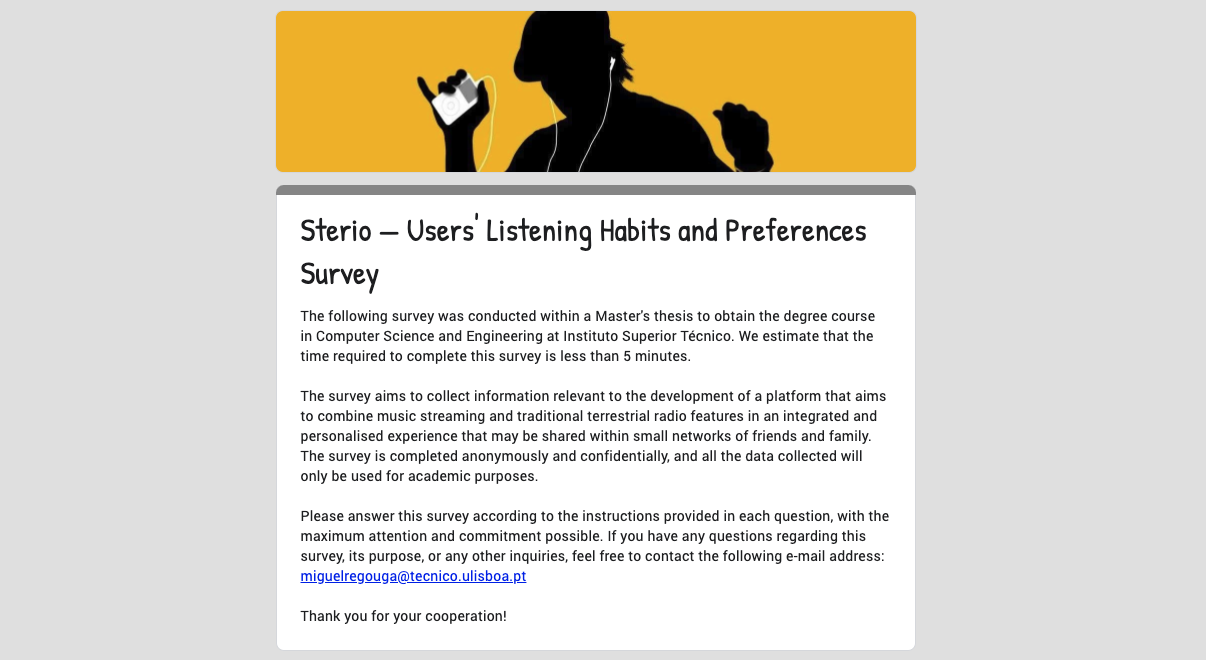
\includegraphics[width=0.8\textwidth]{./Images/survey.png}
\caption{Homepage and introduction to the conducted survey}
\label{fig:test_env}
\end{figure}

Among demographic and other miscellaneous user characterization questions, the following set of queries were asked:

\begin{itemize}
  \item How often do you listen to music?
  \item Which mediums do you use regularly to listen to music?
  \item How often do you use streaming services?
  \item Which music streaming service is your most used one?
  \item On average, how long do you use streaming services in a listening session?
  \item Which of these factors do you consider more relevant when using a streaming service?
  \item What are the factors that stop you from using streaming services on a more regular basis?
  \item Do you listen regularly to podcasts?
  \item How often do you listen to traditional radio stations?
  \item On average, how long do you typically listen to radio?
  \item Where do you usually listen to radio?
  \item What are the main reasons that make you listen to radio stations?
  \item What are the factors that stop you from listening to radio stations on a more regular basis?
\end{itemize}

When asked how often they use music streaming services, only 7\% replied that they don't use them, and \textbf{almost 60\% use them every day}. \textbf{Spotify} is the most used streaming service amongst them, while YouTube (which many use as a means of a streaming service) comes in second place. Users value these services' \textbf{wide range of music selection}, \textbf{sound quality}, and \textbf{low price}, but 16.7\% of them still prefer to use another medium.

\begin{figure}
	\centering
	\caption{Which of these factors do you consider more relevant when using a music streaming service?}
	\begin{bchart}[step=10,max=80,unit=\%,width=0.8\textwidth]
        \bcbar[text=Sound quality]{59.3}
            \smallskip
        \bcbar[text=Wide range of music selection]{71.2}
            \smallskip
        \bcbar[text= Convenience]{68}
            \smallskip
        \bcbar[text=To discover new music]{52.5}
            \smallskip
        \bcbar[text=Curated playlists]{32}
    \end{bchart}
\end{figure}


Regarding traditional terrestrial radio stations, 40.6\% of the inquired listen to them daily, with 5.9\% not listening to this medium at all. Almost half of the inquirers state that the main reason that makes them listen to radio stations is the \textbf{disclosure of news, weather, and traffic information}, with \textbf{convenience} and the \textbf{good mood of the radio hosts} following in second and third places respectively. On the downside, users don't listen to radio more frequently since they believe the music selection is too repetitive (58.2\%) or doesn't fit their taste (40.1\%); due to the high rate of advertisement breaks (50.8\%); and because they can't choose what they want to listen to (38.4\%).

\begin{figure}
	\centering
	\caption{What are the main reasons that make you listen to radio stations?}
	\begin{bchart}[step=10,max=45,unit=\%,width=0.8\textwidth]
        \bcbar[text=Listening to news/weather/traffic information]{41.3}
            \smallskip
        \bcbar[text=Convenience]{37.4}
            \smallskip
        \bcbar[text=Good mood of radio hosts]{33}
            \smallskip
        \bcbar[text=Radio shows]{17.3}
            \smallskip
        \bcbar[text=Other]{11.2}
    \end{bchart}
\end{figure}



\begin{figure}
	\centering
	\caption{What are the factors that stop you from listening to radio stations on a more regular basis?}
	\begin{bchart}[step=10,max=70,unit=\%, width=0.8\textwidth]
        \bcbar[text=Music is too repetitive]{58.1}
            \smallskip
        \bcbar[text=Music does not fit my taste]{40.2}
            \smallskip
        \bcbar[text=Too many ad breaks]{50.8}
            \smallskip
        \bcbar[text=Can't choose what to listen]{38.7}
            \smallskip
        \bcbar[text=Other]{14.6}
    \end{bchart}
\end{figure}


From this first set of gathered data, we can arrive at some early conclusions. The first one is that music streaming services are really popular among this set of users, mainly because they see the advantage of having the possibility on-demand selection of music artists, songs, and genres. However, regarding radio stations, users enjoy the role of the radio host and the disclosure of information this medium provides, but often don't enjoy the music selection nor the long advertisement breaks.

As surveys allow us to reach a larger number of people, the use of this user research method may be a favorable first-step to start user research procedures. To obtain more detailed data about the users' audio media consumption habits, we have also conducted a diary study and interviews, so we could gather qualitative data and cross-reference it with the information obtained through surveying.

\section{Diary study}

To take a deeper look into audio media users' music streaming and traditional terrestrial radio habits, we conducted a diary study, which asks participants to capture information about their activities, habits, thoughts, or opinions as they go about their daily activities. ~\cite{Courage2005} This method allows the collection of typically longitudinal data \textit{in situ}. 

In order to obtain more raw and personal details regarding their audio consuming habits, we involved our own family and friends circle from the very beginning of the project, so we could understand how we can target and improve their experience. As we'll further discuss, we also want to understand how our solution could tackle the social presence and online community concepts, as described by Wang et. al ~\cite{Wang2014}.

We selected 11 close friends and family to conduct a diary study over one week (the participating users on all user research activities are reported in table ~\ref{tab:users}). From these users, 9 are paid subscribers of a music streaming service, while the other 2 use the free tier plan (if available). Users were asked to fill out a template spreadsheet on the Google Sheets~\footnote{For more information, visit the \href{http://sheets.google.com/}{Google Sheets website}.} platform at the end of each day. The template, shown in fig. \ref{fig:diarystudy} and presented in Appendix ~\ref{chapter:appendixB}, had a set of pre-specified questions or probes for users to respond to, making this a structured diary study. Users were asked to sign an informed consent form, presented in Appendix ~\ref{chapter:appendixC}, informing them how their data would be used and the importance of it in regards to the development of our platform.


\begin{figure}[h]
\centering
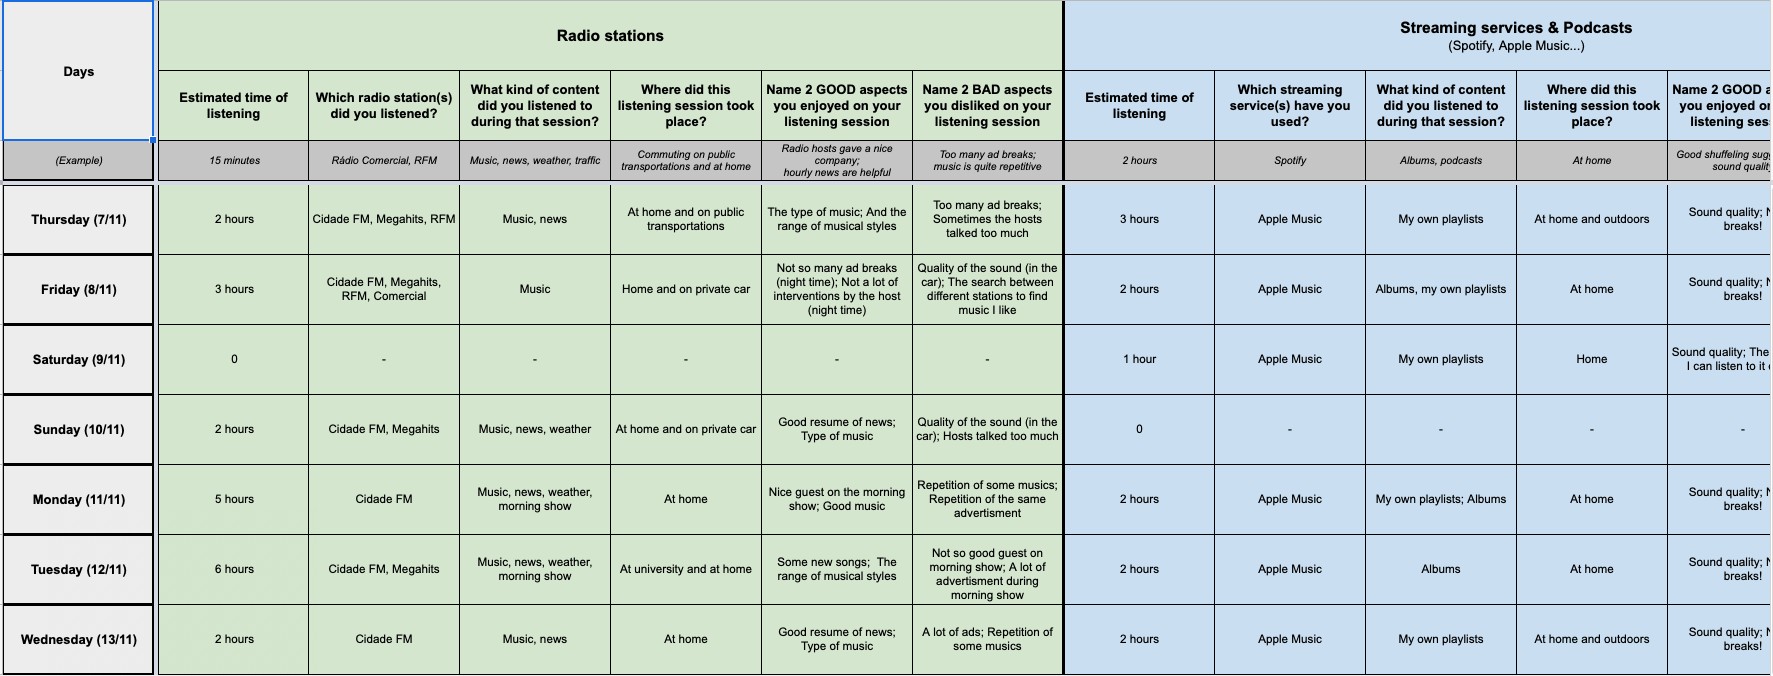
\includegraphics[width=0.8\textwidth]{./Images/diarystudy.png}
\caption{Diary study spreadsheet template filled by one user}
\label{fig:diarystudy}
\end{figure}


The diary study focused on four main audio listening mediums: traditional terrestrial radio stations, music streaming services, music videos, and physical format. Each medium had the following questions:

\begin{itemize}
  \item Estimated time of listening (in minutes);
  \item What kind of content did you listened to during that session?
  \item Where did this listening session took place?
  \item Name two good aspects you enjoyed on your listening session;
  \item Name two bad aspects you disliked on your listening session.
\end{itemize}

From this study, we can analyze both quantitative and qualitative data. Regarding the first, we have concluded that, on average, every user spends more than 3 hours per day listening to various audio content; streaming services count for about 62\% of that, while traditional radio stations count for 21\%. From the 11 users, 2 didn't use music streaming services during that week and are non-paid subscribers, and 3 didn't listen to traditional radio stations in the same period. 

The main outcome of this diary study was, however, qualitative data. For the analysis of such data, we used an \textbf{affinity diagram} ~\cite{Wilson2012}. In an affinity diagram, researchers extract the data from each participant, pulling out key points, and write each note individually on an index card or sticky note. ~\cite{Courage2005} Similar findings or concepts are then grouped to identify themes or trends in the data. 

Affinity diagrams can add structure to a large or complicated issue, as they can break it down either into broader categories or more specific, focused categories. This assists and guides designers in the process of identifying issues that affect multiple areas, making affinity diagrams a crucial tool for organizing qualitative data into themes that may offer insights for the design and testing. ~\cite{Holtzblatt1988} Figure \ref{fig:diagram1} illustrates the first iteration of the affinity diagram created based on this study's participants' data.

\begin{figure}[h]
\centering
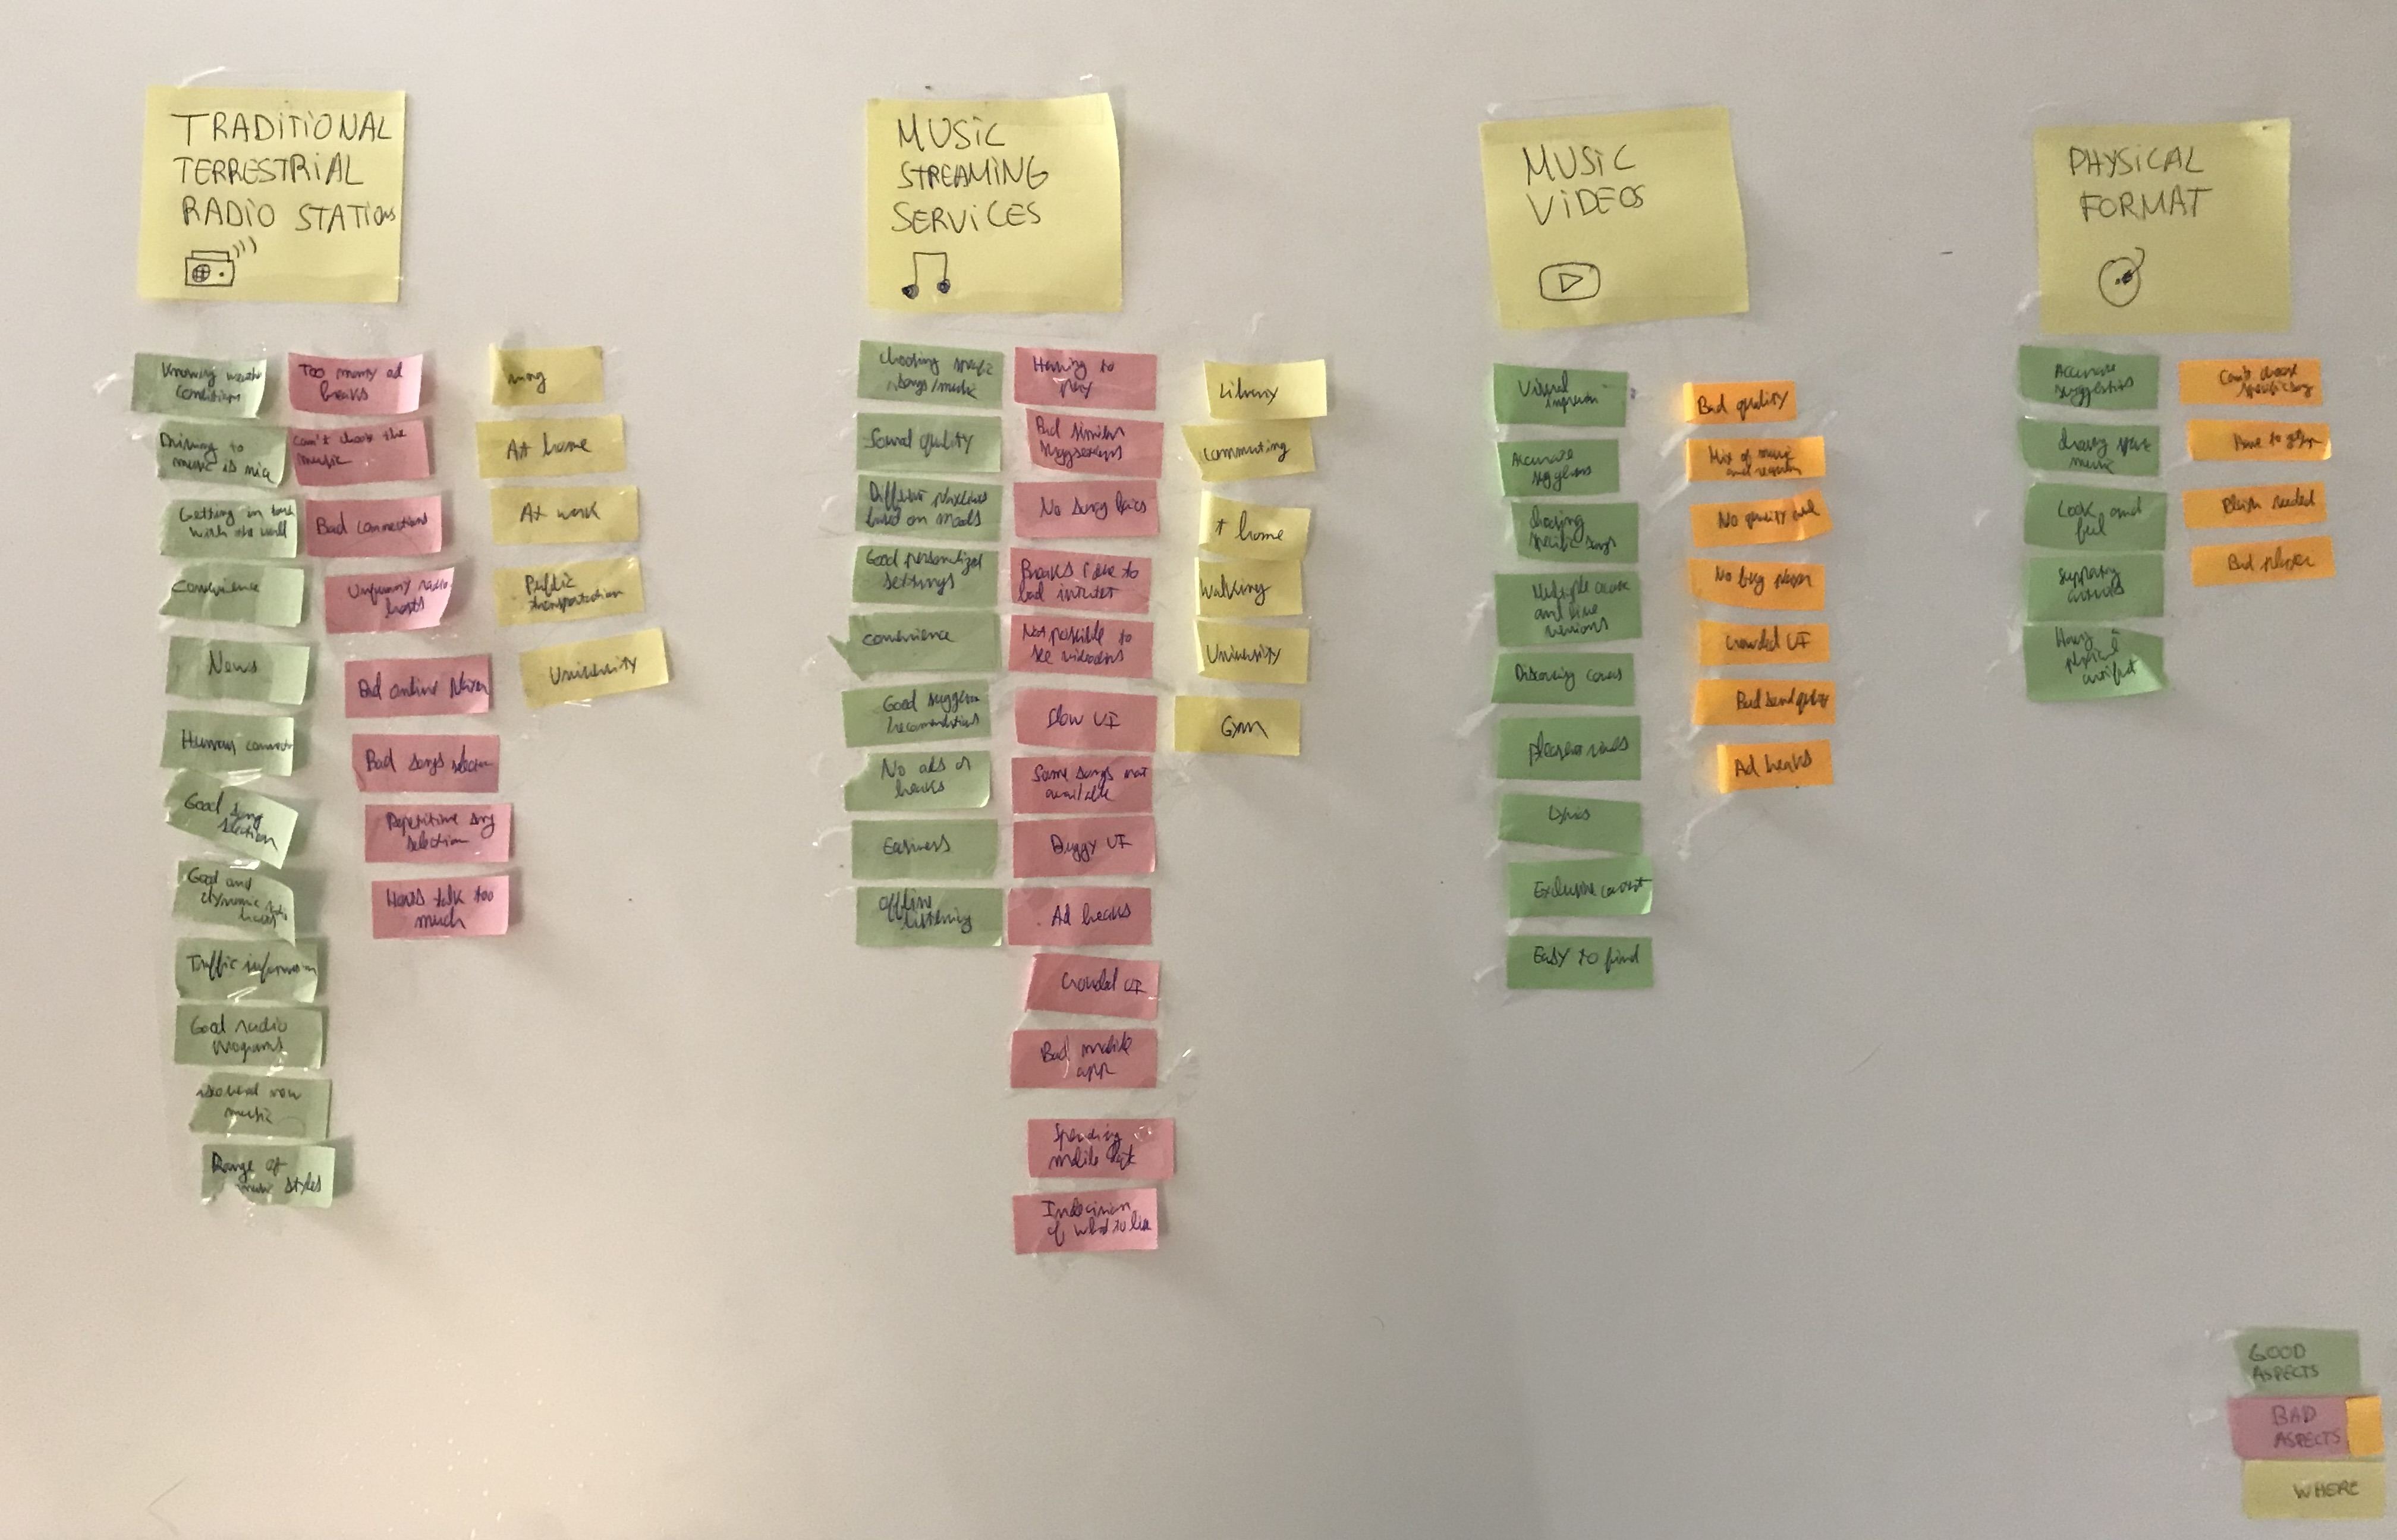
\includegraphics[width=0.8\textwidth]{./Images/affinitydiagram.jpg}
\caption{Affinity diagram with the gathered data from the diary study}
\label{fig:diagram1}
\end{figure}


From the analysis of this data, some conclusions emerge. Regarding traditional terrestrial radio, users enjoy the human connection it provides and the dynamics of the radio hosts. The disclosure of information such as news, weather, and traffic reports is also very important when it comes to listening to radio, as well as the diversity of radio shows that are broadcast. On the downside, most radio listeners of this study don't like the song selection of the stations, as they find it very repetitive, always of the same genre, or simply not matching their musical taste. Not being able to choose what they want to listen to on the radio is something that frustrates them, as well as the amount of radio advertisement breaks.

In contrast, users value the \textbf{freedom of music choice} in music streaming services, as well as its overall \textbf{sound quality} and \textbf{convenience}. They appreciate the \textbf{automatically generated playlists} based on their mood or even their taste. The added freedom that music streaming services provide sometimes isn't a great feature to some users, as they sometimes have indecision of what to listen to (corroborating the tyranny of choice concept discussed in chapter ~\ref{chap:ttr}). 

The diary study has proven to be a great method to gather detailed information about audio media consumers' music streaming and traditional terrestrial radio habits — in conjunction with surveys, a broader dataset is obtained. To finish our preliminary user research, we have conducted interviews, to complement our dataset with information and empathy from our users.

\section{Interviews}

Interviews consist of a guided conversation in which one person seeks information from another. This method is considered flexible and can be conducted as a solo activity or in conjunction with another user experience activity. The result of a set of interviews is an integration of perspectives from multiple users. ~\cite{Courage2005}

We conducted \textbf{semi-structured, in-person} interviews with the 11 participants of the diary study, as a \textbf{follow-up to this method} (the participating users on all user research activities are reported in table ~\ref{tab:users}). We prepared a plan, shown in Appendix ~\ref{chapter:appendixD}, which subdivided the interview into five main sections: \textbf{introduction}, where we encouraged participants to answer honestly and to warn us whenever they couldn't answer one of the questions; \textbf{warm-up}, where the interviewees were asked easy, non-threatening questions in order to get positive answers to ease the participant into the interview; \textbf{body of the session}, where the main questions were asked; \textbf{cooling-off}, asking more general questions to summarize the interview; and \textbf{wrap-up}, where we thanked the interviewees for the time spent with all three user research methods by giving them a small gift.

The main objective of the study was not only to have more detailed information on users' audio media-consuming habits, but also to understand \textbf{how they feel} and \textbf{their opinions} on terrestrial radio and music streaming services. As a semi-structured interview, we begun each section with a set of questions to answer (closed-ended and open-ended), but we also deviated from the order and the set of questions from time to time. Among the planned questions, the following were asked:

\begin{itemize}
  \item What do you enjoy about music streaming services?
  \item What’s your opinion on streaming services’ social capabilities?
  \item When it comes to your music habits, what would you like to share with your friends?
  \item What does music mean to you?
  \item What’s the role of music in in your social life?
  \item What’s your general opinion on traditional radio stations?
  \item Why don’t you listen more often to traditional radio stations?
  \item Which radio stations do you like the most? Why?
  \item What’s your opinion on the role of the radio host?
  \item What do you think about traditional radio stations’ role in news, traffic, or weather disclosure?
\end{itemize}

As with the diary study, we obtained qualitative data from the interviews, which was added (and adapted, when appropriately) it to the previously created affinity diagram (fig. ~\ref{fig:diagram1}). The final affinity diagram, with the gathered data from both the diary study and interviews, is shown in Figure ~\ref{fig:diagram2}.

\begin{figure}[h]
\centering
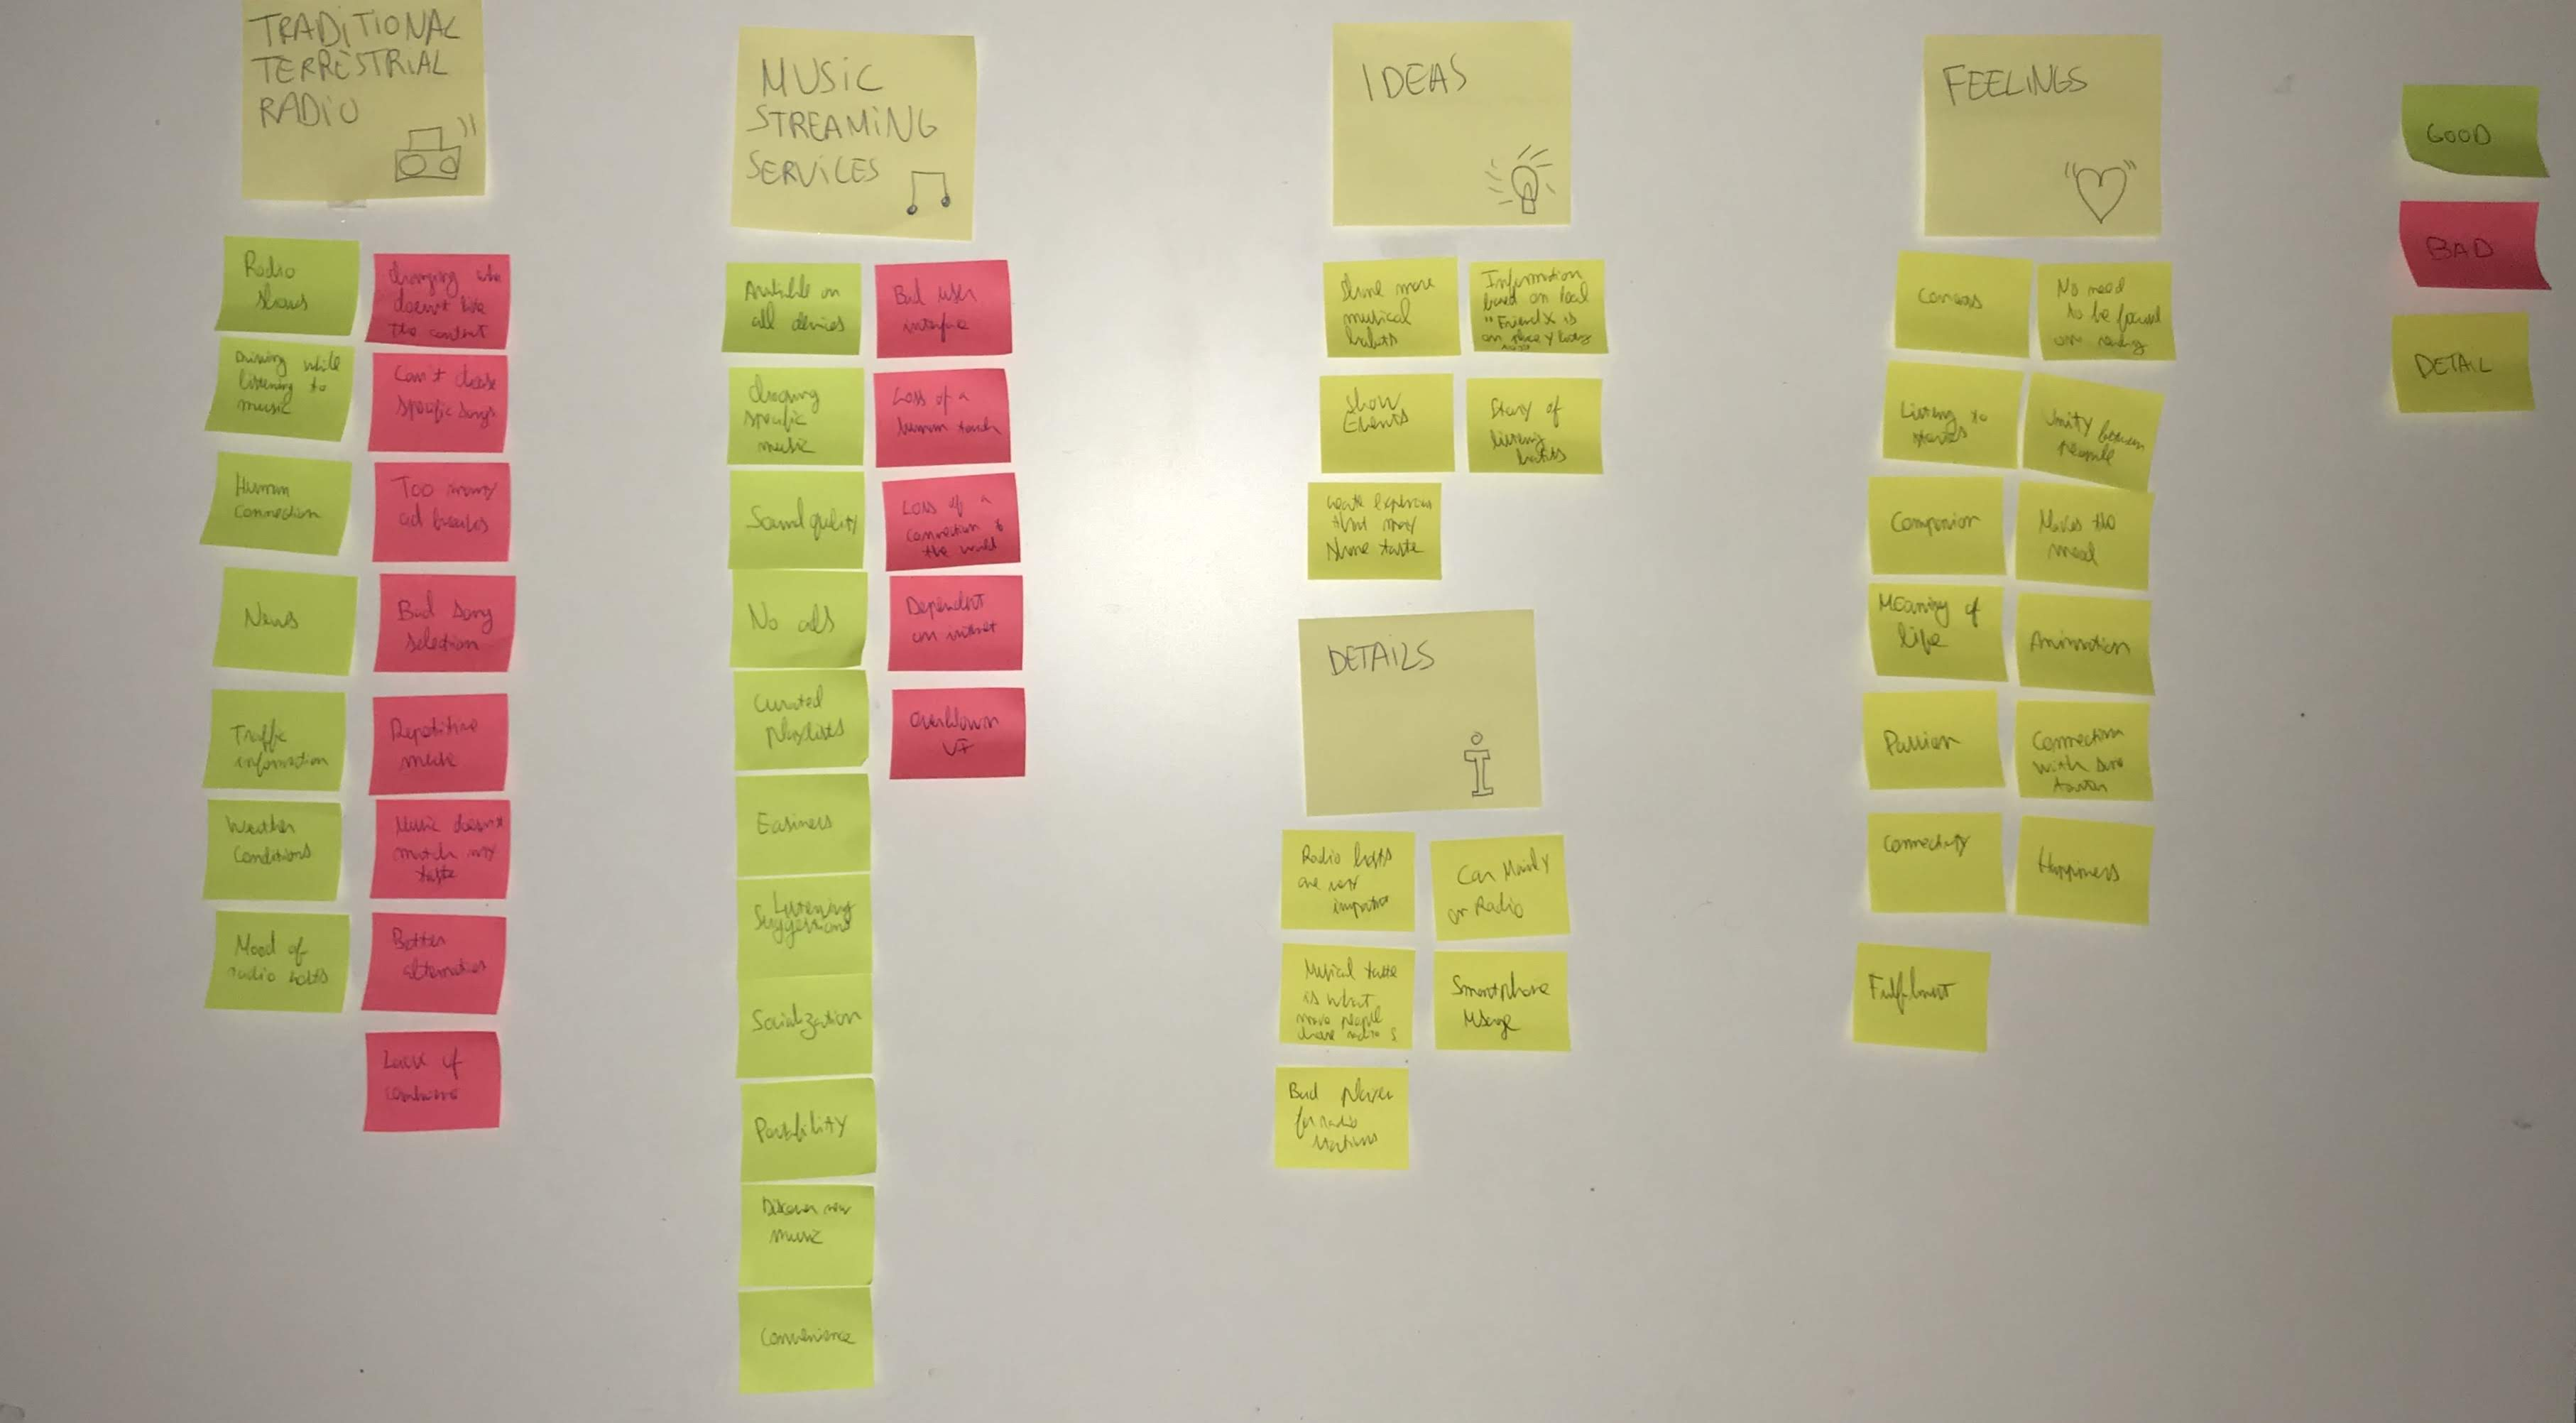
\includegraphics[width=0.8\textwidth]{./Images/finalaffinitydiagram.jpg}
\caption{Final affinity diagram with the gathered data from the diary study and interviews}
\label{fig:diagram2}
\end{figure}

The interviewees have given us important and detailed information regarding their audio consuming habits — how and why they listen to music and other audio content, which factors they value the most and the least in a listening session, and even some ideas and suggestions to implement and take into account when designing our solution. For instance, they noted that the social aspects of music streaming services and terrestrial radio are one of the most important aspects in their listening experience. The expressed empathy will be taken into account when developing the final solution, as all the interviewees expressed that music plays an extremely important role in their routines, and the way they experience it is a pivotal attribute.

To help us explore a diverse group of early-stage concepts, and to reflect on their stature, we will use the speed dating methodology, as proposed by Davidoff et. al ~\cite{Davidoff2007}. Speed dating supports low-cost rapid comparison of design opportunities and situated applications by creating structured, bounded, serial engagements, based on the preliminary user research we delineated in this section. In return, by structuring a comparison of concepts, this method will assist us on the contextualization of multiple applications, as well as of critical aspects of individual applications, helping us in the identification and understanding of contextual risk factors, and how we can develop approaches to address them. Section ~\ref{sec:speeddating} will describe the developed work in the ambit of this concept.